% Chapter Template

\chapter{EDA and classifier performance} % Main chapter title

\label{chapter3} % Change X to a consecutive number; for referencing this chapter elsewhere, use \ref{ChapterX}

\section{EDA}
There are a total of 18,829 annotated sentences and the top 10 frequently occurring practices make up close to 60\% of all sentences (Figure~\ref{fig:eda_data_practice}). The bottom 10 frequently occurring practices make up approximately 1\% of the dataset. There does not seem to be much variation in sentence length for the top 10 frequently occurring practices, since the standard deviation of the mean is approximately 2.5 words and the median 1.9 words across the top 10 practices. This is also seen by similar interquartile range (IQR) (Figure~\ref{fig:boxplot_top_10}). The mean of the sentence lengths for all top 10 practices are slightly greater than the median, which suggest some outliers with very long sentence lengths (Figure~\ref{fig:graph_sentence_length}) that cause a slightly right skew distribution (Figure~\ref{fig:hist}). The distributions are also unimodal, with the mode around 20. Similar sentence length could indicate similar sentence complexity across the practices. 

% \begin{table}[!ht]
% 	\resizebox{\textwidth}{!}{
% 	\begin{tabular}{lrrrr}
% 	\toprule
% 									  practice &  counts &  mean sentence length &  median sentence length &  percentage of total \\
% 	\midrule
% 	Identifier\_Cookie\_1stParty &    2107 &             25.4 &                    22.0 &           11.2\% \\
% 			   Contact\_E\_Mail\_Address\_1stParty &    2106 &             28.7 &                    25.0 &           11.2\% \\
% 							 Location\_1stParty &    1514 &             29.2 &                    24.0 &           8.1\% \\
% 	Identifier\_Cookie\_Tech\_3rdParty &    1250 &             27.3 &                    24.0 &           6.6\% \\
% 				Identifier\_IP\_Address\_1stParty &    1005 &             30.9 &                    27.0 &           5.3\% \\
% 				 Contact\_Phone\_Number\_1stParty &     970 &             29.1 &                    25.0 &           5.2\% \\
% 				 Identifier\_Device\_ID\_1stParty &     697 &             32.4 &                    28.0 &           3.7\% \\
% 			   Contact\_Postal\_Address\_1stParty &     597 &             28.9 &                    26.0 &           3.2\% \\
% 										   SSO &     504 &             32.6 &                    28.0 &           2.7\% \\
% 					  Demographic\_Age\_1stParty &     428 &             33.1 &                    26.0 &           2.3\% \\
% 	\bottomrule
% 	\end{tabular}
% 	}
% 	\caption{Summary statistics per practice of top 10 occurring practices.}
% 	\label{tab:top_10_sentence}
% 	\end{table}

\begin{figure}[!ht]
	\centering
	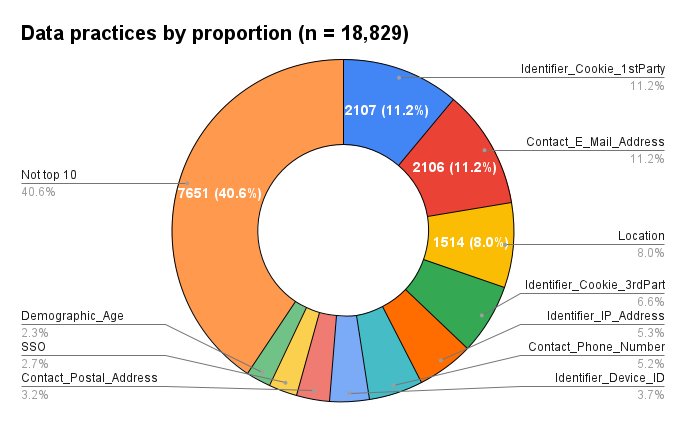
\includegraphics[width=1\textwidth]{figures/eda_data_practices.png}      
    \caption{Breakdown of data practices by proportion}
    \label{fig:eda_data_practice}
\end{figure}

% \begin{table}[!ht]
% 	\centering
% 	\begin{tabular}{lrr}
% 		\toprule
% 		{} &  Mean sentence length &  Median sentence length \\
% 		\midrule
% 		count &             10.0 &               10.0 \\
% 		mean  &             29.8 &               25.5 \\
% 		std   &              2.5 &                1.9 \\
% 		min   &             25.4 &               22.0 \\
% 		25\%   &             28.7 &               24.3 \\
% 		50\%   &             29.1 &               25.5 \\
% 		75\%   &             32.0 &               26.8 \\
% 		max   &             33.1 &               28.0 \\
% 		\bottomrule
% 	\end{tabular}
% 	\caption{Summary statistics of sentence length of the top 10 occurring practices.}
% 	\label{tab:summary_top_10_practices}
% \end{table}

\begin{figure}[!ht]
	\centering
	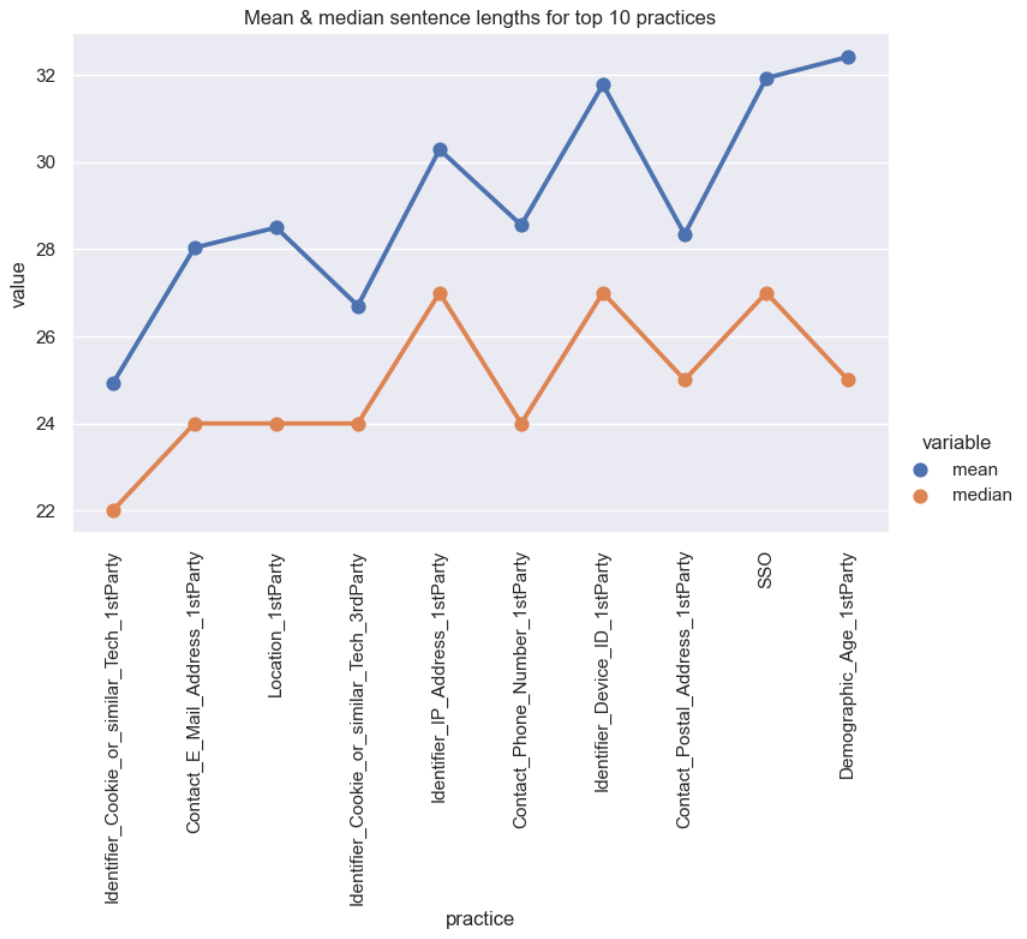
\includegraphics[width=1\textwidth]{figures/eda_mean_median.png}      
    \caption{Mean and median sentence length}
    \label{fig:graph_sentence_length}
\end{figure}


\begin{figure}[!ht]
	\begin{subfigure}[t]{.5\linewidth}
	  \centering
	  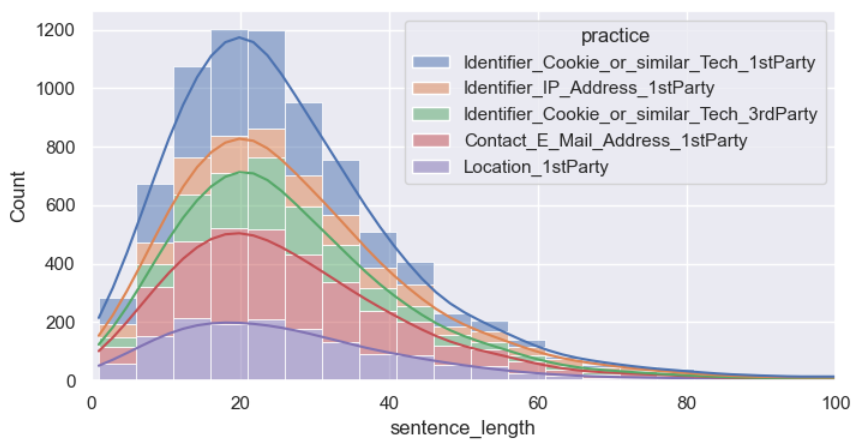
\includegraphics[width=1\linewidth]{figures/hist_eda.png}
	  \caption{Histogram of top 5 practices}
	  \label{fig:hist}
	\end{subfigure}
	\hfill
	\begin{subfigure}[t]{.5\linewidth}
		\centering
		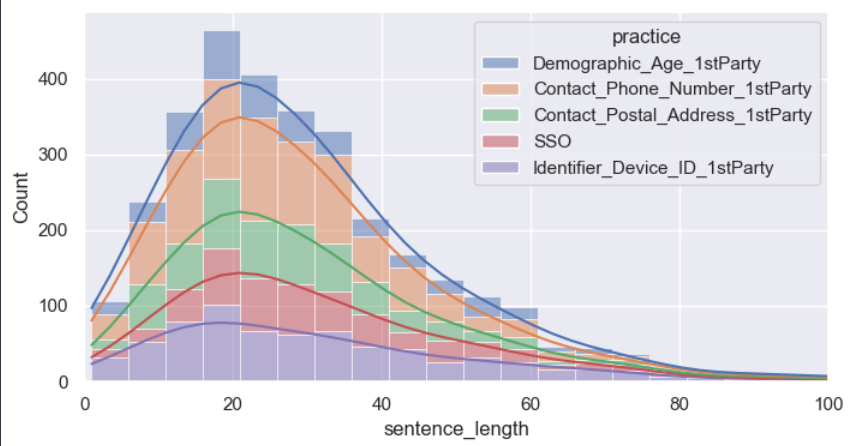
\includegraphics[width=1\linewidth]{figures/hist_eda_2.png}
		\caption{Histogram of next top 5 practices}
		\label{fig:hist_2}
	\end{subfigure}
	\medskip
	\begin{subfigure}[b]{1\linewidth}
	  \centering
	  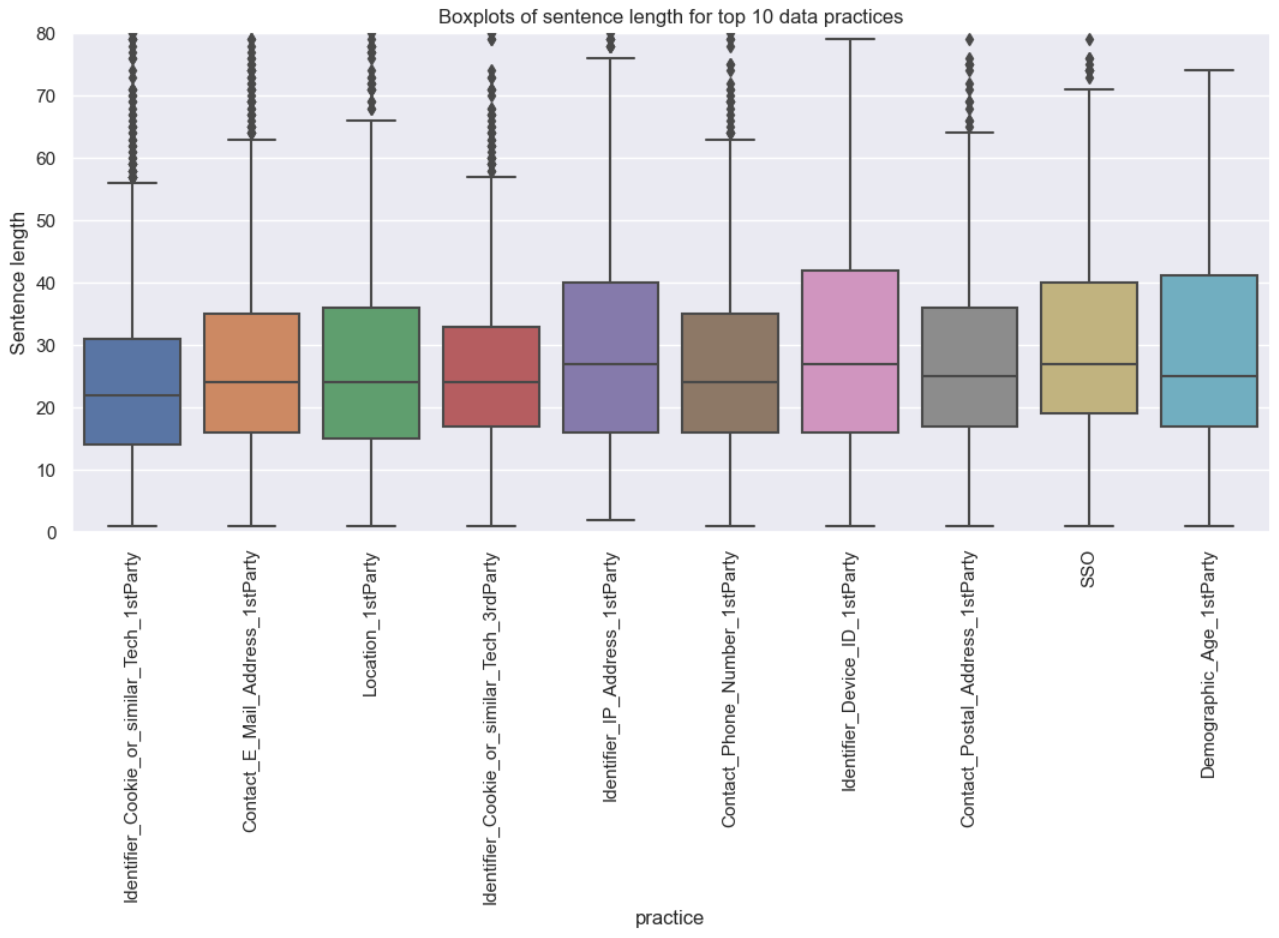
\includegraphics[width=0.85\linewidth]{figures/eda_boxplots.png}
	  \caption{Boxplots of sentence length (Practices shown in order of descending frequency)}
	  \label{fig:boxplot_top_10}
	\end{subfigure}
	\caption{Summary plots for top 10 frequently occurring data practices (note: not all outliers shown to focus on visualising IQR)}
	\label{fig:eda}
\end{figure}

With regard to top 10 frequently occurring 4-grams in the top 5 practices (Figure~\ref{fig:4_grams_sentence}), both 4-grams of \texttt{Cookie 1st Party} and \texttt{Cookie 3rd Party} contain many instances of "cookies" across their top 10 occurring 4-grams. It is difficult to tell from the 4-grams alone whether the sentences refer to collection of cookies by 1st or 3rd parties. The same is seen to a lesser extent between the 4-grams of \texttt{Location} and \texttt{IP Address}, where both have instances of "IP address" and "mac address". Such similar 4-grams could affect the separability of the classes. In comparison, 4-grams of \texttt{Email} are clearly distinct from the rest of the data practices with unique tokens of "email" and "phone number". 

\begin{figure}[!ht]
	\begin{subfigure}[t]{.5\textwidth}
	  \centering
	  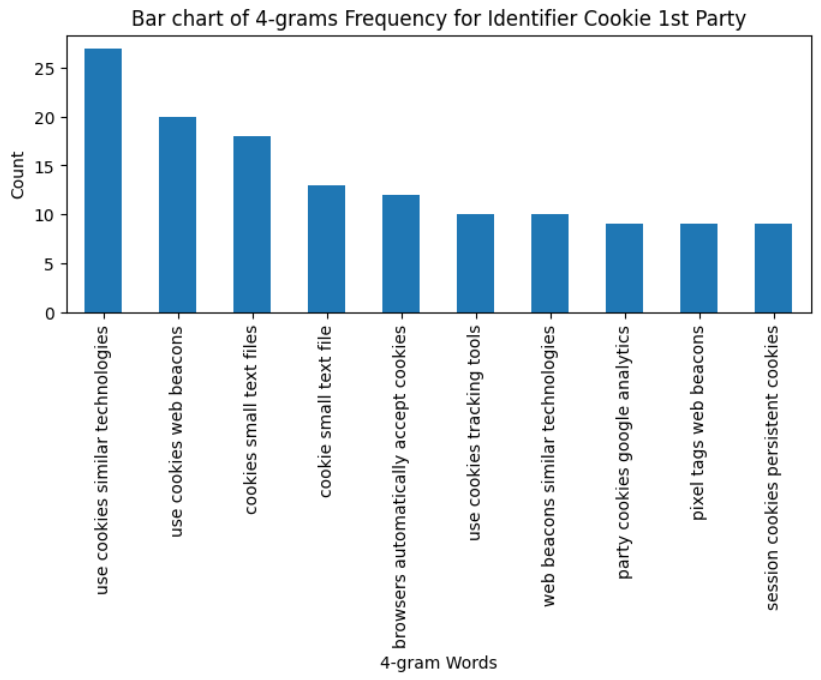
\includegraphics[width=\linewidth]{figures/4_grams_cookie_1stParty.png}
	  \caption{Identifier Cookie 1st Party}
	\end{subfigure}
	\hfill
	\begin{subfigure}[t]{.5\textwidth}
	  \centering
	  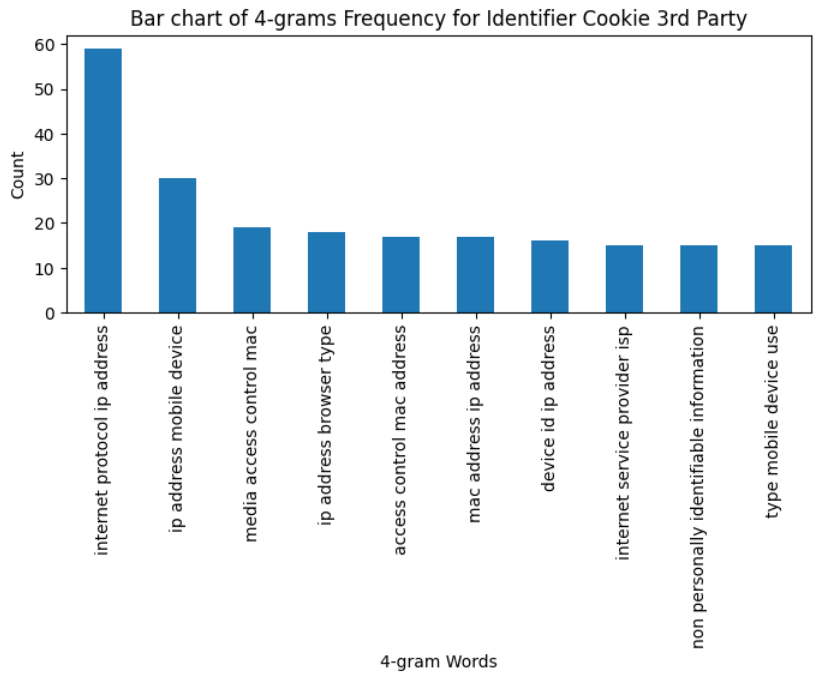
\includegraphics[width=\linewidth]{figures/4_grams_cookie_3rdParty.png}
	  \caption{Identifier Cookie 3rd Party}
	\end{subfigure}
	
	\medskip
  
	\begin{subfigure}[t]{.5\textwidth}
	  \centering
	  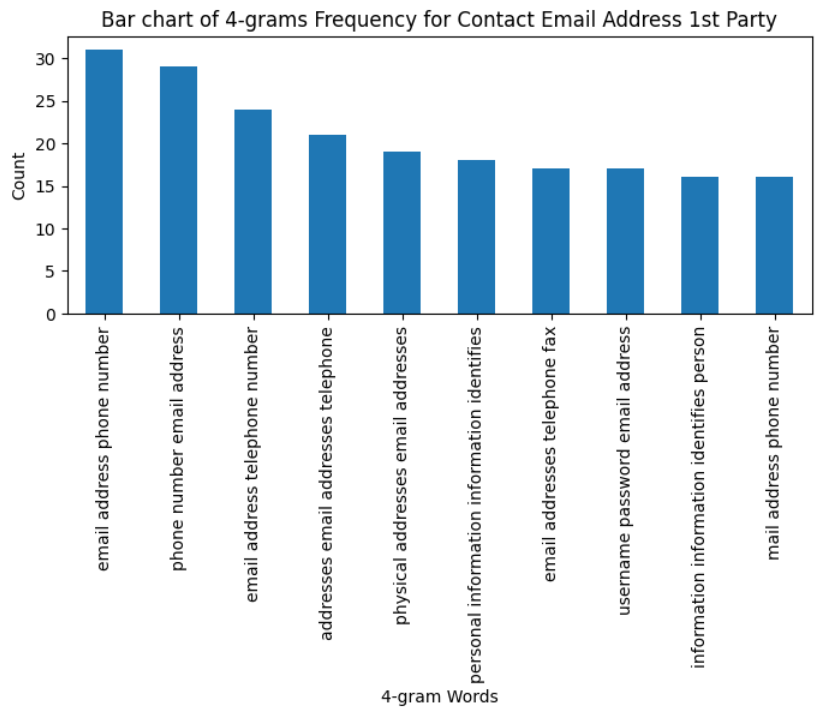
\includegraphics[width=\linewidth]{figures/4_grams_email.png}
	  \caption{Identifier Email}
	\end{subfigure}
	\hfill
	\begin{subfigure}[t]{.5\textwidth}
	  \centering
	  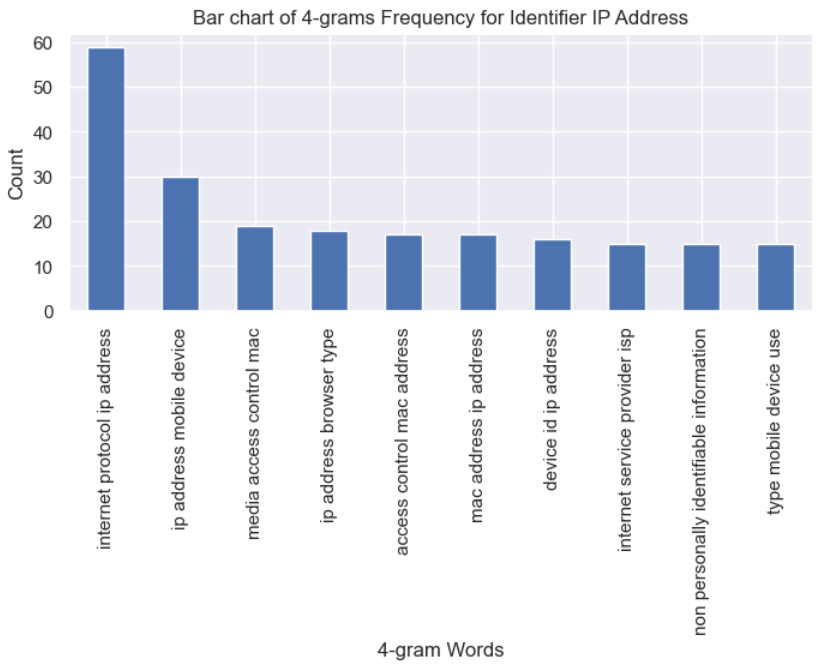
\includegraphics[width=\linewidth]{figures/4_grams_ip_address.png}
	  \caption{Identifier IP Address}
	\end{subfigure}
	\begin{subfigure}[t]{.5\textwidth}
		\centering
		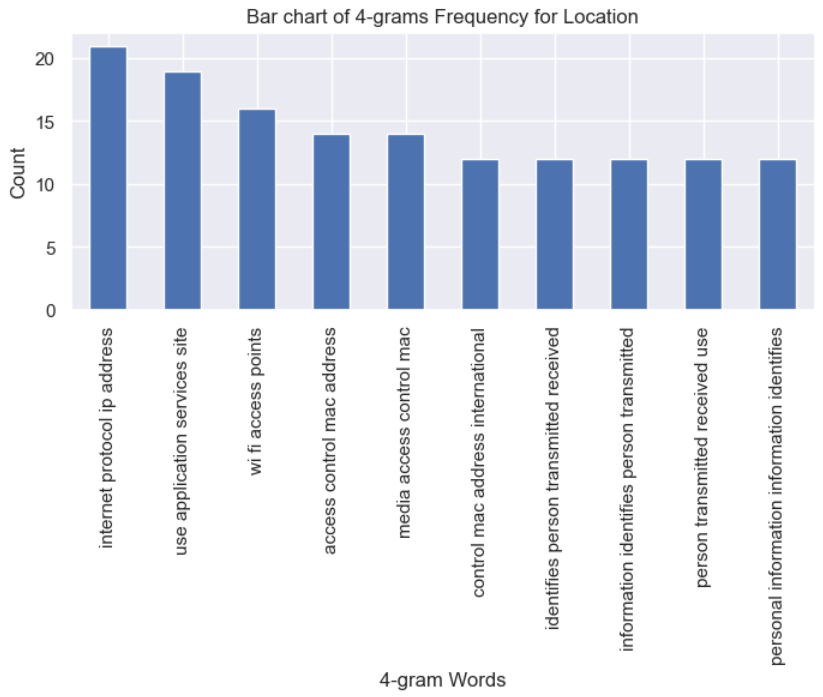
\includegraphics[width=\linewidth]{figures/4_grams_location.png}
		\caption{Location 1st Party}
	\end{subfigure}
	\caption{Top 10 most frequently occurring 4-grams in the top most frequently occurring 5 data practices at the sentence level}
	\label{fig:4_grams_sentence}
  \end{figure}

\section{Performance of classifiers for top N practices}
I compare the weighted precision, recall and F1 scores of the classifiers below. Since there is neither a high risk of identifying false positives or false negatives, F1 score is primarily used to assess the performance of the classifiers. As there is class imbalance in the top 10 data practices (Table~\ref{fig:eda_data_practice}), I focus on the weighted average F1 scores as the most important indicator of classifier performance. All classifiers were trained using one-vs-the-rest strategy for computational efficiency.

Given that there are in total 57 practices for the entire dataset but the top 10 data practices already comprise 60\% of all sentences, training classifiers on all 57 practices would likely lead to low performance. Thus, to find an optimal balance between classifier performance but still maintain realistic problem space for classification, I first assess the performance of the three classifiers using Tf-IDF for the top N (where $3 \le N \le 10$) frequently occurring practices. SVC consistently performs the best across the metrics and across the top N frequently occurring practices (Figure~\ref{fig:top_n_practices}). This corresponds with the findings by \cite{zimmeck2019}. Also, performance of all the classifiers generally decreases with increasing $N$, which is not surprising since it is more difficult for the classifier to find a decision boundary with more classes. The following sections focuses on classifier performance of the top 5 practices as performance was still reasonable at 60\% weighted P/R/F1 scores. Also, since SGDClassifier performed the worst compared to the 2 other classifiers, I focus only on comparing logistic regression and SVC, with logistic regression as a baseline classifier.

\begin{figure}[!ht]
	\centering
	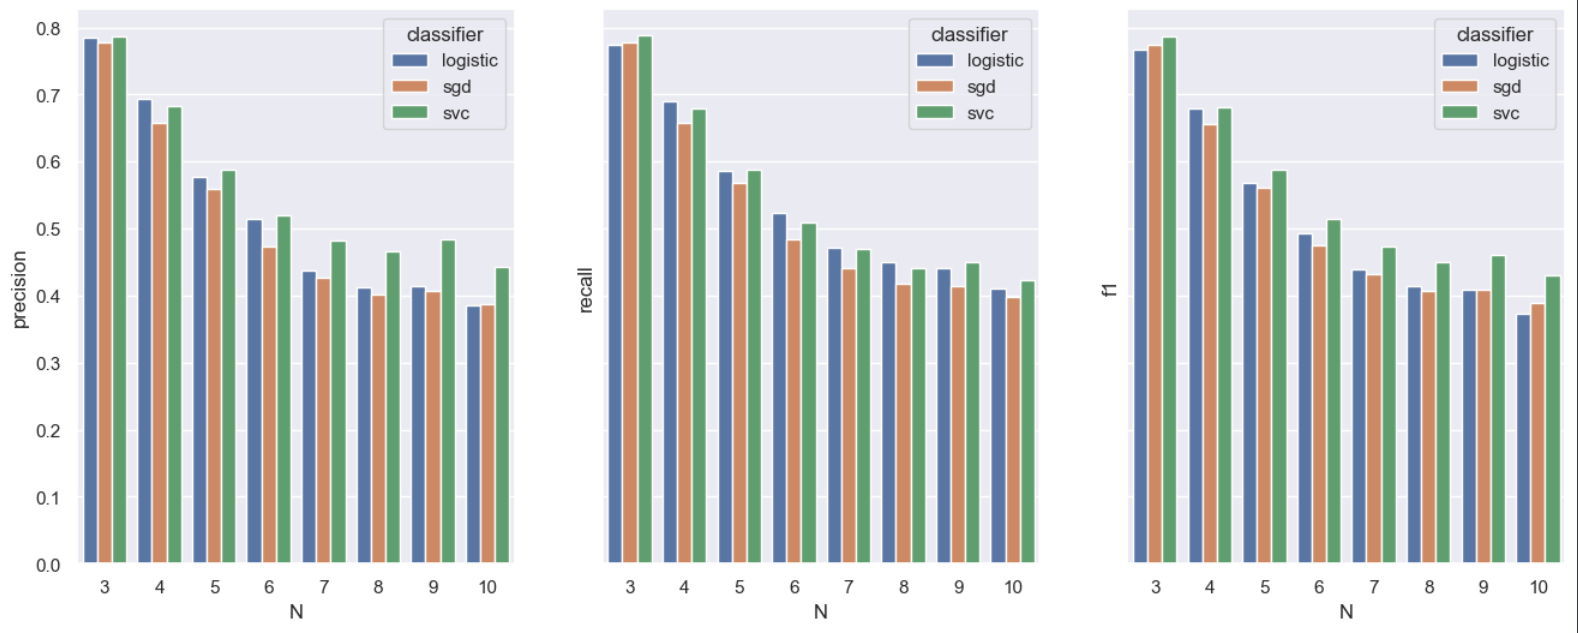
\includegraphics[width=1\textwidth]{figures/model_n_testing_sentence.png}      
    \caption{Weighted average P/R/F1 scores for top N ($3 \le N \le 10$) practices}
    \label{fig:top_n_practices}
\end{figure}

\section{Performance of individual classifiers for top 5 practices}
\label{sec:perf_top_5}
I report the individual performance of all 4 combinations of text representations and models. With regard to P/R/F1 scores (Figure~\ref{fig:heatmaps_perf}), similarly to what \cite{zimmeck2019} found, SVC + Tf-IDF provided the best overall performance with the weighted average at 66\%. This is a significant performance difference from the lowest performing model, logistic regression + GloVe at 54\%. Specifically for \texttt{Cookie 1st Party}, both logistic regression + Tf-IDF and SVC + Tf-IDF performed similarly at 68\% F1, but SVC + Tf-IDF had a more balanced performance across precision and recall. With regard to the ROC curves (Figure~\ref{fig:roc_curve}), looking at the micro-averaged AUC, the classifiers all performed similarly well within a small difference of 0.03. Similarly for \texttt{Cookie 1st Party}, the difference in AUC was insignificant at 0.02. Interestingly, GloVe embeddings seem to cause a greater variance when comparing the AUC for each class. For instance, the difference between the highest and lowest AUC for logistic regression + GloVe is $0.89 - 0.77 = 0.12$, while for logistic regression + Tf-IDF it was $0.91 - 0.85 = 0.06$.

In terms of performance for the individual classes, \texttt{Email Address} consistently performed the best across the classifiers, followed by \texttt{Cookie 1st Party}, \texttt{Location}, \texttt{IP Address} and \texttt{Cookie 3rd Party}. The difference in performance between the top performing class \texttt{Email Address} and \texttt{Cookie 3rd Party} can be up to 33\% difference in weighted F1 depending on the classifier used. Specific class performance for \texttt{Cookie 1st Party} varied quite significantly from 68\% using SVC + Tf-IDF, to 55\% for SVC + GloVe. The performance differences of the classes might be accounted for by the uniqueness of the top 10 frequently occurring 4-grams as mentioned above. Since the 4-grams of \texttt{Email} were the most distinct compared to the rest, the classifiers could more easily separate \texttt{Email} from the rest of the classes which resulted in highest performance.

Overall, these performance figures confirm that SVC is the better performing model, though the performance difference between the benchmark logistic regression and SVC is not that significant (from 62\% to 66\% weighted average F1 when comparing between the classifiers that both use Tf-IDF). Further, the choice of text representation seemed to affect performance more than the choice of model. This is because GloVe embeddings performed worse and caused higher variance in performance compared to Tf-IDF regardless of the model used, when GloVe is the more sophisticated text representation that can capture the semantic meaning of the tokens. These results correspond with a study measuring performance of supervised machine learning for classification tasks using generalised text datasets \cite{hsu2020}, where LinearSVC followed by logistic regression were the highest performing models. 


\begin{figure}[!ht]
	\begin{subfigure}[t]{.5\textwidth}
	  \centering
	  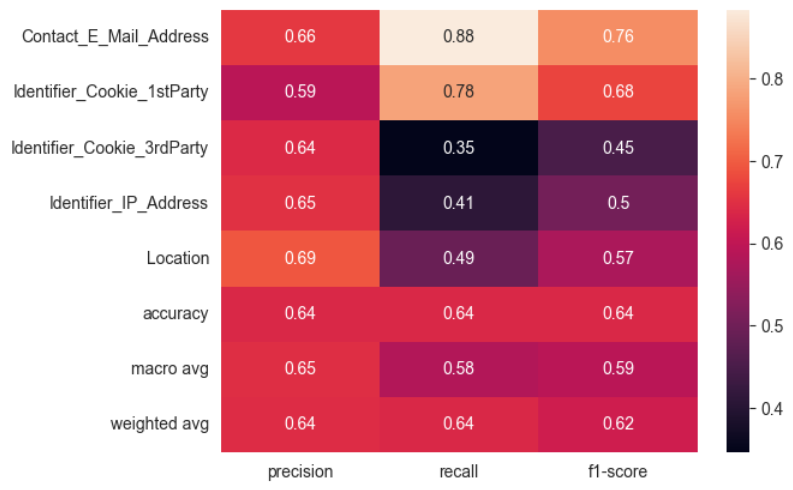
\includegraphics[width=\linewidth]{figures/heatmap_log_tfidf.png}
	  \caption{Logistic regression + TfIDF}
	\end{subfigure}
	\hfill
	\begin{subfigure}[t]{.5\textwidth}
	  \centering
	  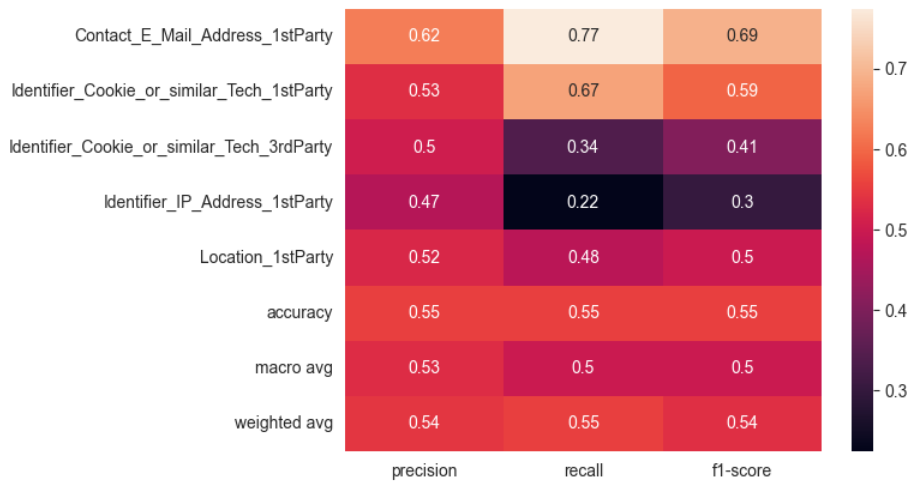
\includegraphics[width=\linewidth]{figures/heatmap_log_glove.png}
	  \caption{Logistic regression + GloVe}
	\end{subfigure}
	
	\medskip
  
	\begin{subfigure}[t]{.5\textwidth}
	  \centering
	  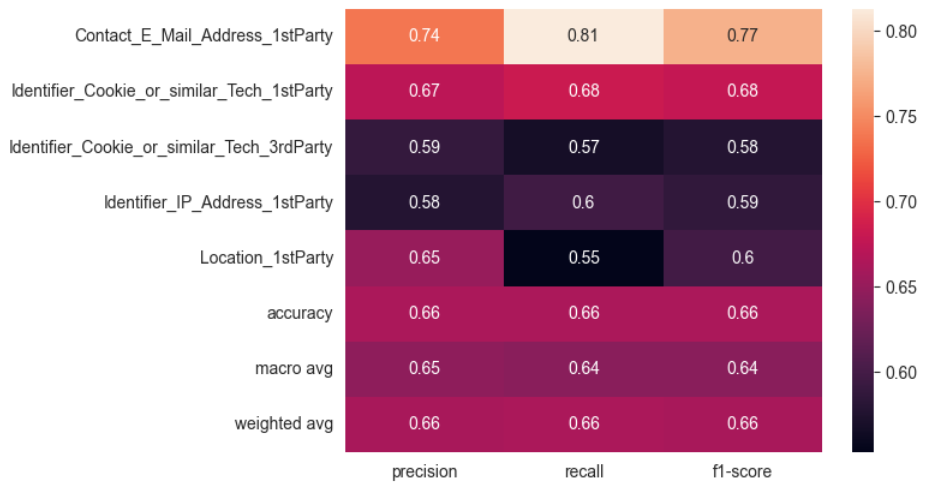
\includegraphics[width=\linewidth]{figures/heatmap_svc_tfidf.png}
	  \caption{SVC + TfIDF}
	\end{subfigure}
	\hfill
	\begin{subfigure}[t]{.5\textwidth}
	  \centering
	  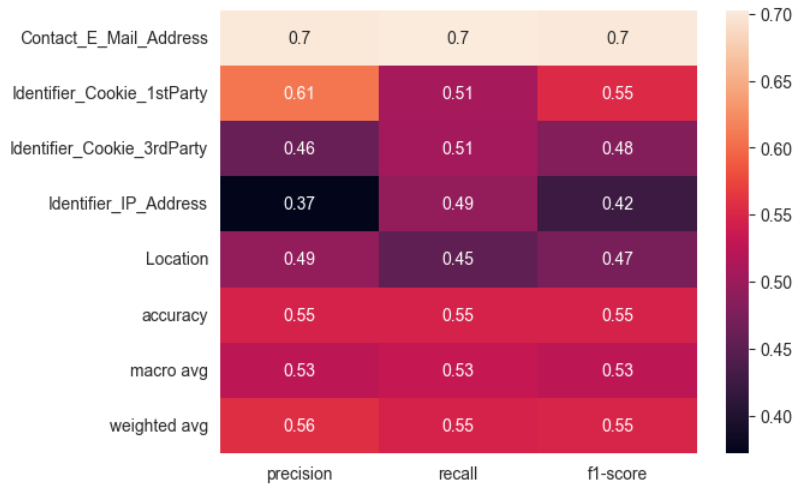
\includegraphics[width=\linewidth]{figures/heatmap_svc_glove.png}
	  \caption{SVC + GloVe}
	\end{subfigure}
	\caption{Performance heatmaps of the 4 classifiers (averaged over 5-fold cross validation)}
	\label{fig:heatmaps_perf}
  \end{figure}

\begin{figure}[!ht]
	\begin{subfigure}[t]{.5\textwidth}
	  \centering
	  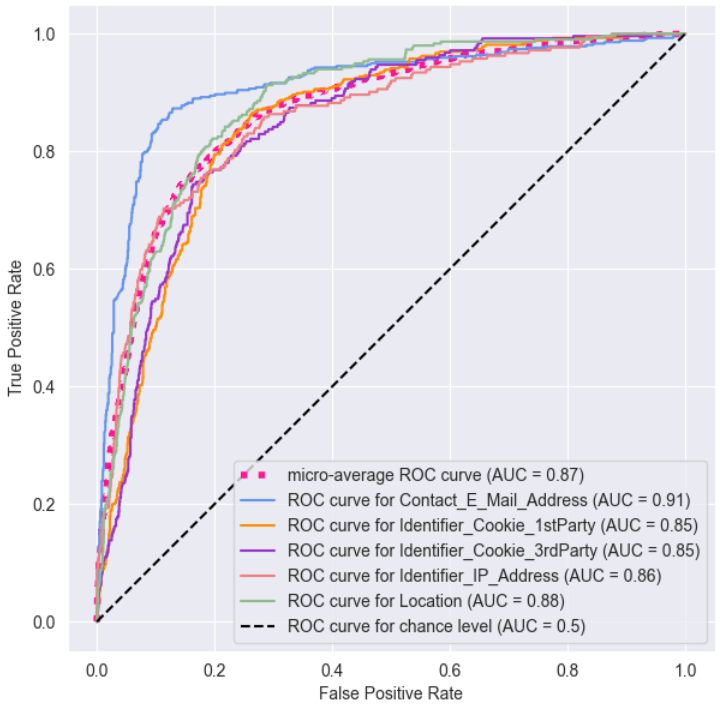
\includegraphics[width=\linewidth]{figures/roc_logistic_tfidf.png}
	  \caption{Logistic regression + TfIDF}
	\end{subfigure}
	\hfill
	\begin{subfigure}[t]{.5\textwidth}
	  \centering
	  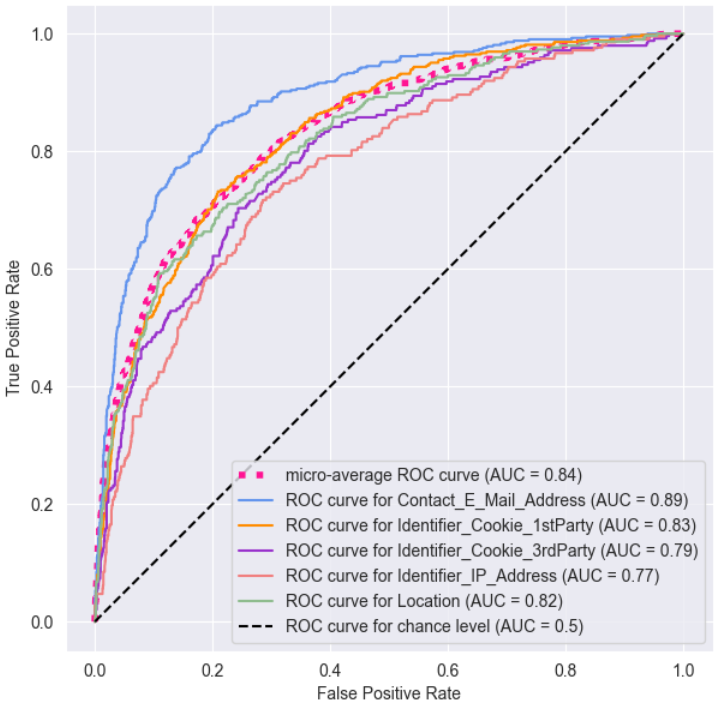
\includegraphics[width=\linewidth]{figures/roc_logistic_glove.png}
	  \caption{Logistic regression + GloVe}
	\end{subfigure}
	
	\medskip
  
	\begin{subfigure}[t]{.5\textwidth}
	  \centering
	  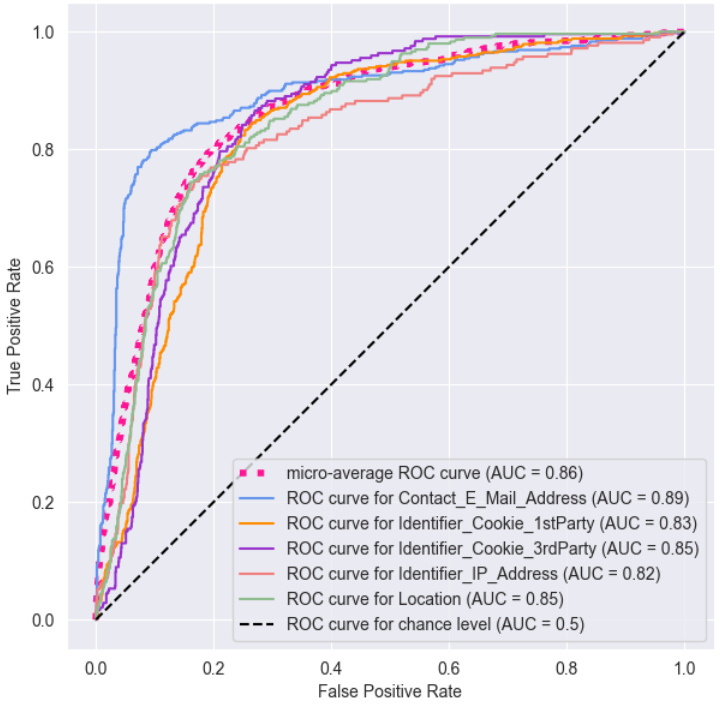
\includegraphics[width=\linewidth]{figures/roc_svc_tfidf.png}
	  \caption{SVC + TfIDF}
	\end{subfigure}
	\hfill
	\begin{subfigure}[t]{.5\textwidth}
	  \centering
	  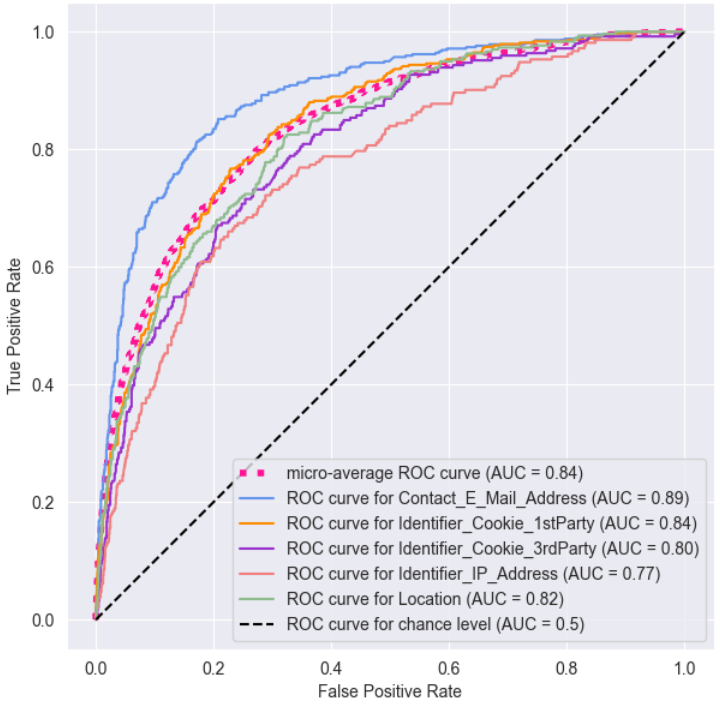
\includegraphics[width=\linewidth]{figures/roc_svc_glove.png}
	  \caption{SVC + GloVe}
	\end{subfigure}
	\caption{Multiclass Receiver Operating Characteristic (ROC) Curve of the 5 data practices for each classifier}
	\label{fig:roc_curve}
  \end{figure}


% 	\begin{table}[!ht]
% 		\resizebox{\textwidth}{!}{
% 		\begin{tabular}{lrrrr}
% 		\toprule
% 								practice &  counts &  sentence\_length\_mean &  sentence\_length\_median &  counts\_percentage \\
% 		\midrule
% 		Identifier\_Mobile\_Carrier\_3rdParty &      35 &             47.1 &                    30.0 &           0.19\% \\
% 					Contact\_ZIP\_3rdParty &      34 &             40.2 &                    41.0 &           0.18\% \\
% 		Identifier\_SSID\_BSSID\_1stParty &      33 &             28.1 &                    24.0 &           0.18\% \\
% 			  Contact\_Password\_3rdParty &      33 &             24.2 &                    20.0 &           0.18\% \\
% 					Contact\_City\_3rdParty &      24 &             180 &                    14.0 &           0.13\% \\
% 		Contact\_Address\_Book\_3rdParty &      17 &             39.6 &                    34.0 &           0.1\% \\
% 			  Identifier\_IMSI\_1stParty &      13 &             48.2 &                    44.0 &           0.07\% \\
% 		Identifier\_SIM\_Serial\_3rdParty &       5 &             41.2 &                    54.0 &           0.03\% \\
% 			  Identifier\_IMSI\_3rdParty &       4 &             54.3 &                    47.5 &           0.02\% \\
% 		Identifier\_SSID\_BSSID\_3rdParty &       2 &             65.5 &                    65.5 &           0.01\% \\
% 		\bottomrule
% 	\end{tabular}
% 	}
% 	\caption{Summary statistics for bottom 10 frequently occurring practices.}
% 	\label{tab:bottom_10_sentence}
% \end{table}


% \begin{table}[!ht]
% 	\resizebox{\textwidth}{!}{
% 		\begin{tabular}{lllll}
% 		\hline
% 		\multicolumn{1}{|l|}{\textbf{Data Practice}}          & \multicolumn{1}{l|}{\textbf{Precision}} & \multicolumn{1}{l|}{\textbf{Recall}} & \multicolumn{1}{l|}{\textbf{F1}} & \multicolumn{1}{l|}{\textbf{Support}} \\ \hline
% 		\multicolumn{1}{|l|}{Contact Email Address 1st Party} & \multicolumn{1}{l|}{0.66}               & \multicolumn{1}{l|}{0.88}            & \multicolumn{1}{l|}{0.76}        & \multicolumn{1}{l|}{2106}              \\ \hline
% 		\multicolumn{1}{|l|}{Identifier Cookie 1st Party}    & \multicolumn{1}{l|}{0.59}               & \multicolumn{1}{l|}{0.78}            & \multicolumn{1}{l|}{0.68}        & \multicolumn{1}{l|}{2107}              \\ \hline
% 		\multicolumn{1}{|l|}{Identifier Cookie 3rd Party}     & \multicolumn{1}{l|}{0.64}               & \multicolumn{1}{l|}{0.35}            & \multicolumn{1}{l|}{0.45}        & \multicolumn{1}{l|}{1250}              \\ \hline
% 		\multicolumn{1}{|l|}{Identifier IP Address 1st Party} & \multicolumn{1}{l|}{0.66}               & \multicolumn{1}{l|}{0.41}            & \multicolumn{1}{l|}{0.50}        & \multicolumn{1}{l|}{1005}              \\ \hline
% 		\multicolumn{1}{|l|}{Location 1st Party}              & \multicolumn{1}{l|}{0.69}               & \multicolumn{1}{l|}{0.49}            & \multicolumn{1}{l|}{0.57}        & \multicolumn{1}{l|}{1514}              \\ \hline
% 																&                                         &                                      &                                  &                                       \\ \hline
% 		\multicolumn{1}{|l|}{\textbf{accuracy}}               & \multicolumn{1}{l|}{}                   & \multicolumn{1}{l|}{}                & \multicolumn{1}{l|}{0.64}        & \multicolumn{1}{l|}{7982}             \\ \hline
% 		\multicolumn{1}{|l|}{\textbf{macro avg}}              & \multicolumn{1}{l|}{0.65}               & \multicolumn{1}{l|}{0.58}            & \multicolumn{1}{l|}{0.59}        & \multicolumn{1}{l|}{7982}             \\ \hline
% 		\multicolumn{1}{|l|}{\textbf{weighted avg}}           & \multicolumn{1}{l|}{0.64}               & \multicolumn{1}{l|}{0.64}            & \multicolumn{1}{l|}{0.62}        & \multicolumn{1}{l|}{7982}             \\ \hline
% 		\end{tabular}
% 	}
% 	\caption{Logistic regression + Tf-IDF}
% 	\label{tab:lr+tfidf}
% \end{table}


% \begin{table}[!ht]
% 	\resizebox{\textwidth}{!}{
% 		\begin{tabular}{lllll}
% 		\hline
% 		\multicolumn{1}{|l|}{\textbf{Data Practice}}          & \multicolumn{1}{l|}{\textbf{Precision}} & \multicolumn{1}{l|}{\textbf{Recall}} & \multicolumn{1}{l|}{\textbf{F1}} & \multicolumn{1}{l|}{\textbf{Support}} \\ \hline
% 		\multicolumn{1}{|l|}{Contact Email Address 1st Party} & \multicolumn{1}{l|}{0.62}               & \multicolumn{1}{l|}{0.77}            & \multicolumn{1}{l|}{0.70}        & \multicolumn{1}{l|}{2106}              \\ \hline
% 		\multicolumn{1}{|l|}{Identifier Cookie 1st Party}    & \multicolumn{1}{l|}{0.53}               & \multicolumn{1}{l|}{0.67}            & \multicolumn{1}{l|}{0.59}        & \multicolumn{1}{l|}{2107}              \\ \hline
% 		\multicolumn{1}{|l|}{Identifier Cookie 3rd Party}     & \multicolumn{1}{l|}{0.50}               & \multicolumn{1}{l|}{0.34}            & \multicolumn{1}{l|}{0.41}        & \multicolumn{1}{l|}{1250}              \\ \hline
% 		\multicolumn{1}{|l|}{Identifier IP Address 1st Party} & \multicolumn{1}{l|}{0.47}               & \multicolumn{1}{l|}{0.22}            & \multicolumn{1}{l|}{0.30}        & \multicolumn{1}{l|}{1005}              \\ \hline
% 		\multicolumn{1}{|l|}{Location 1st Party}              & \multicolumn{1}{l|}{0.52}               & \multicolumn{1}{l|}{0.48}            & \multicolumn{1}{l|}{0.50}        & \multicolumn{1}{l|}{1514}              \\ \hline
% 																&                                         &                                      &                                  &                                       \\ \hline
% 		\multicolumn{1}{|l|}{\textbf{accuracy}}               & \multicolumn{1}{l|}{}                   & \multicolumn{1}{l|}{}                & \multicolumn{1}{l|}{0.55}        & \multicolumn{1}{l|}{7982}             \\ \hline
% 		\multicolumn{1}{|l|}{\textbf{macro avg}}              & \multicolumn{1}{l|}{0.53}               & \multicolumn{1}{l|}{0.50}            & \multicolumn{1}{l|}{0.50}        & \multicolumn{1}{l|}{7982}             \\ \hline
% 		\multicolumn{1}{|l|}{\textbf{weighted avg}}           & \multicolumn{1}{l|}{0.54}               & \multicolumn{1}{l|}{0.55}            & \multicolumn{1}{l|}{0.54}        & \multicolumn{1}{l|}{7982}             \\ \hline
% 		\end{tabular}
% 	}
% 	\caption{Logistic regression + GloVe embeddings}
% 	\label{tab:lr+glove}
% \end{table}


% \begin{table}[!ht]
% 	\resizebox{\textwidth}{!}{
% 	\begin{tabular}{lllll}
% 		\hline
% 		\multicolumn{1}{|l|}{\textbf{Data Practice}}          & \multicolumn{1}{l|}{\textbf{Precision}} & \multicolumn{1}{l|}{\textbf{Recall}} & \multicolumn{1}{l|}{\textbf{F1}} & \multicolumn{1}{l|}{\textbf{Support}} \\ \hline
% 		\multicolumn{1}{|l|}{Contact Email Address 1st Party} & \multicolumn{1}{l|}{0.74}               & \multicolumn{1}{l|}{0.81}            & \multicolumn{1}{l|}{0.77}        & \multicolumn{1}{l|}{2106}              \\ \hline
% 		\multicolumn{1}{|l|}{Identifier Cookie 1st Party}     & \multicolumn{1}{l|}{0.67}               & \multicolumn{1}{l|}{0.68}            & \multicolumn{1}{l|}{0.68}        & \multicolumn{1}{l|}{2107}              \\ \hline
% 		\multicolumn{1}{|l|}{Identifier Cookie 3rd Party}     & \multicolumn{1}{l|}{0.59}               & \multicolumn{1}{l|}{0.57}            & \multicolumn{1}{l|}{0.58}        & \multicolumn{1}{l|}{1250}              \\ \hline
% 		\multicolumn{1}{|l|}{Identifier IP Address 1st Party} & \multicolumn{1}{l|}{0.58}               & \multicolumn{1}{l|}{0.60}            & \multicolumn{1}{l|}{0.59}        & \multicolumn{1}{l|}{1005}              \\ \hline
% 		\multicolumn{1}{|l|}{Location 1st Party}              & \multicolumn{1}{l|}{0.65}               & \multicolumn{1}{l|}{0.55}            & \multicolumn{1}{l|}{0.60}        & \multicolumn{1}{l|}{1514}              \\ \hline
% 																&                                         &                                      &                                  &                                       \\ \hline
% 		\multicolumn{1}{|l|}{\textbf{accuracy}}               & \multicolumn{1}{l|}{}                   & \multicolumn{1}{l|}{}                & \multicolumn{1}{l|}{0.66}        & \multicolumn{1}{l|}{7982}             \\ \hline
% 		\multicolumn{1}{|l|}{\textbf{macro avg}}              & \multicolumn{1}{l|}{0.65}               & \multicolumn{1}{l|}{0.64}            & \multicolumn{1}{l|}{0.64}        & \multicolumn{1}{l|}{7982}             \\ \hline
% 		\multicolumn{1}{|l|}{\textbf{weighted avg}}           & \multicolumn{1}{l|}{0.66}               & \multicolumn{1}{l|}{0.66}            & \multicolumn{1}{l|}{0.66}        & \multicolumn{1}{l|}{7982}             \\ \hline
% 		\end{tabular}
% 	}
% 	\caption{SVC + Tf-IDF}
% 	\label{tab:svc+tfidf}
% \end{table}

% \begin{table}[!ht]
% 	\resizebox{\textwidth}{!}{
% 	\begin{tabular}{lllll}
% 		\hline
% 		\multicolumn{1}{|l|}{\textbf{Data Practice}}          & \multicolumn{1}{l|}{\textbf{Precision}} & \multicolumn{1}{l|}{\textbf{Recall}} & \multicolumn{1}{l|}{\textbf{F1}} & \multicolumn{1}{l|}{\textbf{Support}} \\ \hline
% 		\multicolumn{1}{|l|}{Contact Email Address 1st Party} & \multicolumn{1}{l|}{0.70}               & \multicolumn{1}{l|}{0.70}            & \multicolumn{1}{l|}{0.70}        & \multicolumn{1}{l|}{2106}              \\ \hline
% 		\multicolumn{1}{|l|}{Identifier Cookie 1st Party}     & \multicolumn{1}{l|}{0.61}               & \multicolumn{1}{l|}{0.51}            & \multicolumn{1}{l|}{0.55}        & \multicolumn{1}{l|}{2107}              \\ \hline
% 		\multicolumn{1}{|l|}{Identifier Cookie 3rd Party}     & \multicolumn{1}{l|}{0.46}               & \multicolumn{1}{l|}{0.51}            & \multicolumn{1}{l|}{0.48}        & \multicolumn{1}{l|}{1250}              \\ \hline
% 		\multicolumn{1}{|l|}{Identifier IP Address 1st Party} & \multicolumn{1}{l|}{0.37}               & \multicolumn{1}{l|}{0.49}            & \multicolumn{1}{l|}{0.42}        & \multicolumn{1}{l|}{1005}              \\ \hline
% 		\multicolumn{1}{|l|}{Location 1st Party}              & \multicolumn{1}{l|}{0.49}               & \multicolumn{1}{l|}{0.45}            & \multicolumn{1}{l|}{0.47}        & \multicolumn{1}{l|}{1514}              \\ \hline
% 																&                                         &                                      &                                  &                                       \\ \hline
% 		\multicolumn{1}{|l|}{\textbf{accuracy}}               & \multicolumn{1}{l|}{}                   & \multicolumn{1}{l|}{}                & \multicolumn{1}{l|}{0.55}        & \multicolumn{1}{l|}{7982}             \\ \hline
% 		\multicolumn{1}{|l|}{\textbf{macro avg}}              & \multicolumn{1}{l|}{0.53}               & \multicolumn{1}{l|}{0.53}            & \multicolumn{1}{l|}{0.53}        & \multicolumn{1}{l|}{7982}             \\ \hline
% 		\multicolumn{1}{|l|}{\textbf{weighted avg}}           & \multicolumn{1}{l|}{0.56}               & \multicolumn{1}{l|}{0.55}            & \multicolumn{1}{l|}{0.55}        & \multicolumn{1}{l|}{7982}             \\ \hline
% 	\end{tabular}
% 	}
% 	\caption{SVC + GloVe embeddings}
% 	\label{tab:svc+glove}
% \end{table}